\documentclass[10pt]{extarticle} % Usa fonte de 10pt
\usepackage{graphicx} % Required for inserting images
\usepackage{float}
\usepackage{geometry}
\usepackage{hyperref}
\usepackage{minted}
\usepackage{bookmark}
\setminted{
  breaklines=true, % Permite quebra de linha
  breakanywhere=true, % Permite quebra em qualquer posição
  fontsize=\small % Define tamanho da fonte para ajudar com overflow
}

\geometry{margin=1in}

\title{Trabalho de Implementação 3 - Heurísticas e Metaheurísticas}
\author{Francisco Teixeira Rocha Aragão - 2021031726}

\date{Data: Dezembro de 2024}

\begin{document}

\maketitle

\section{Introdução}

O presente trabalho busca resolver de maneira aproximada o problema do caixeiro viajante (TSP), fazendo uso da metaheurística GRASP como implementação. Como o problema pertence a classe NP, faz-se necessário o uso de tais estratégias, sendo utilizado no trabalho uma heurística construtiva randomizada adaptativa para definição do caminho inicial, além de diferentes funções de vizinhança para implementar a busca local durante as iterações. Abaixo encontra-se mais informações sobre a implementação além dos resultados obtidos.

\section{Heurísticas utilizadas}

Primeiramente sobre a heurística utilizada, a estratégia implementada para definição inicial de uma solução refere-se a uma heurística construtiva, ou seja, uma heurística em que a solução é construída do zero, desde o início até a resolução do problema. Iniciando-se assim de uma solução vazia, obtendo então uma solução parcial a cada iteração em que ao final é transformada em uma solução completa válida.

Desse modo, a estratégia utilizada foi baseada em uma abordagem gulosa, em que a cada ponto (ou cidade), o próximo trajeto escolhido é aquele com a menor distância. O início é feito a partir de uma cidade (será explicado mais frente) e a cada iteração novas cidades são adicionadas no caminho até todas as cidades serem visitadas, voltando assim ao vértice inicial resolvendo o problema. Com isso, garante-se a validade da solução retornada, em que a cada iteração acrescenta-se uma nova cidade não visitada anteriormente, terminando o algoritmo até visitar a última cidade, retornando ao ponto inicial. Sobre o ponto inicial escolhido, pode tanto iniciar da primeira cidade quanto da cidade central, sendo escolhida a segunda por apresentar melhores resultados na prática. Vale destacar que a estratégia implementada possui um alto custo, embora seja simples, sendo necessário encontrar todas as distâncias a partir do nó atual para os vizinhos, ordenar essas distâncias para então o próximo candidato ser escolhido da lista restrita. Como o grafo é completo, todos os vizinhos estão ligados em todos, com o custo sendo O(n) pois todos os nós são percorridos, O(n) para olhar todos os vizinhos de cada nó e O(nlogn) para ordenar os vizinhos, totalizando O(n²) para a construção do caminho inicial.

A implementação dessa estratégia construtiva foi um pouco alterada no GRASP, tendo em vista o caráter randomizado da metaheurística. Assim, a cada iteração é feita uma escolha aleatória entre as cidades disponíveis, de modo a evitar soluções presas em ótimos locais. Além disso, a escolha aleatória é feita a partir de uma lista de candidatos, que possui tamanho adaptativo de acordo com o nó atual, podendo ter um tamanho pequeno caso os possíveis próximos nós forem muito diferentes, ou um tamanho maior caso sejam parecidos. Isso é feito utilizando a fórmula L = c\_min - alpha * (c\_max - c\_min) em que c\_min e c\_max são as menores e maiores distâncias para o próximo vizinho, alpha é um fator de ajuste e L é o tamanho da lista de candidatos. Com isso, a cada iteração é feita uma escolha aleatória entre os candidatos, de modo a diversificar as soluções encontradas.

Após isso, foi implementada a busca local utilizando diferentes vizinhanças, semelhante a ideia de VND, cujo obtivo é, após encontrar uma primeira solução, utilizar diferentes funções de vizinhanças para melhorar a solução obtida, com as diferentes vizinhanças ajudando a diversificar as soluções. Para isso foram utilizado 2 funções de vizinhança diferentes, sendo elas a troca de 2 cidades e a troca de 3 cidades. A troca de 2 cidades (2-opt, com complexidade O(n²)) funciona trocando apenas dois caminhos da solução inicial, enquanto a troca de 3 cidades (3-opt, com complexidade O(n³)) troca 3 caminhos. Para a estratégia da busca local, é utilizada a abordagem melhor aprimorante, em que ao encontrar um vizinho melhor, automaticamente a busca nessa vizinhança é retomada, buscando encotrar o ótimo local em cada vizinhança antes de passar para a próxima. 

Com isso, todo o processo ocorre buscando a primeira solução através da estratégia gulosa randomizada, e após isso é feita a busca local utilizando as diferentes vizinhanças. Ao final, uma solução é encontrada e armazeanda, com uma nova iteração sendo feita, repetindo o processo até o número de limites de iterações, garantindo assim a diversificação das soluções encontradas com o GRASP.

\section{Execução e Resultados}

O código foi desenvolvido em C++ e os testes foram realizados em uma máquina com debian 12, 16GB de ram e processador I5-11 geração. Sua execução pode ser realizada com os seguintes comandos:

\begin{minted}{c++}
// compilação
make

// limpar arquivos gerados
make clean

// rodar programa
make run ARGS="<pasta instâncias de entrada> <tipo da cidade inicial> <alpha> <iteracoes>"
// <tipo de cidade inicial> = 0 para usar a primeira cidade e 1 para usar cidade central
// idealmente <alpha> deve ser entre 0 e 1
\end{minted}

Vale destacar que os arquivos de entrada foram encontrados no site TSPLIB95, presente nas referências no trabalho, com o projeto executando apenas as instâncias que terminam com a extensão '.tsp'. Além disso, a execução foi realizada diferentes vezes para cada instância, com as médias dos resultados disponíveis nas tabelas abaixo. Essa abordagem é importante visto o caráter randomizado do GRASP, em que a cada iteração é feita uma escolha aleatória, podendo assim variar o resultado final.  

Desse modo, observando as imagens 1 e 2 presentes abaixo, é possível visualizar os resultados do GRASP para as instâncias de teste utilizadas, sendo alpha igual a 0 e 5 iterações. Percebe-se que essa abordagem puramente gulosa apresentou um erro percentual de aproximadamente 10\% para as instâncias menores, e 20\% para as instâncias maiores, embora o erro aumente em alguns casos específicos, podendo estar relacionado a disposição das cidades nessas instâncias. Vale destacar no entanto que o tempo médio de execução é baixo, o tempo segue a tendências de aumentar bem rápido para maiores instâncias. Percebe-se também obseravando a imagem 3 como a diferença entre a solução inicial (heurística construtiva) e a solução final (GRASP) é pequena, o que é justificado pelo alpha ser igual a 0, ou seja, a escolha das cidades é feita de forma gulosa, sem aleatoriedade, levando a resultados melhores inicialmente com menor margem de melhoria com a busca local.

\begin{figure}[H]
    \centering
        \begin{minipage}{0.5\textwidth}
        \centering
        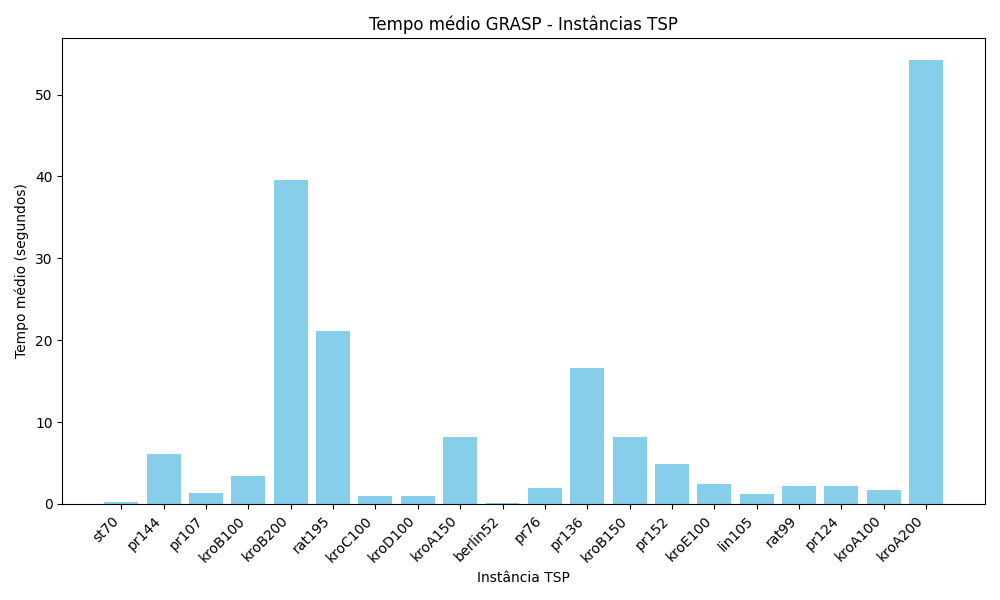
\includegraphics[width=1\textwidth]{./plots/average_times_saida_00_5.log.png}
        \caption{Tempo médio alpha 0 iterações 5}
        \label{fig:Tempo médio alpha 0 iterações 5}
    \end{minipage}\hfill
    \begin{minipage}{0.5\textwidth}
        \centering
        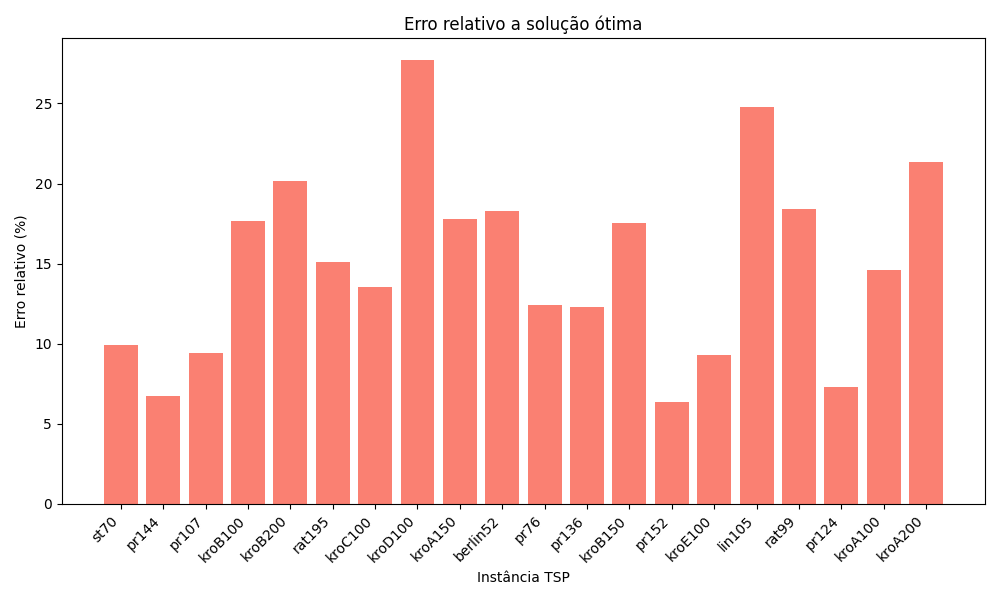
\includegraphics[width=1.0\textwidth]{./plots/solution_comparison_saida_00_5.log.png}
        \caption{Erro percentual alpha 0 iterações 5}
        \label{fig:Erro percentual alpha 0 iterações 5}
    \end{minipage}

\end{figure}

\begin{figure}[H]
    \centering
    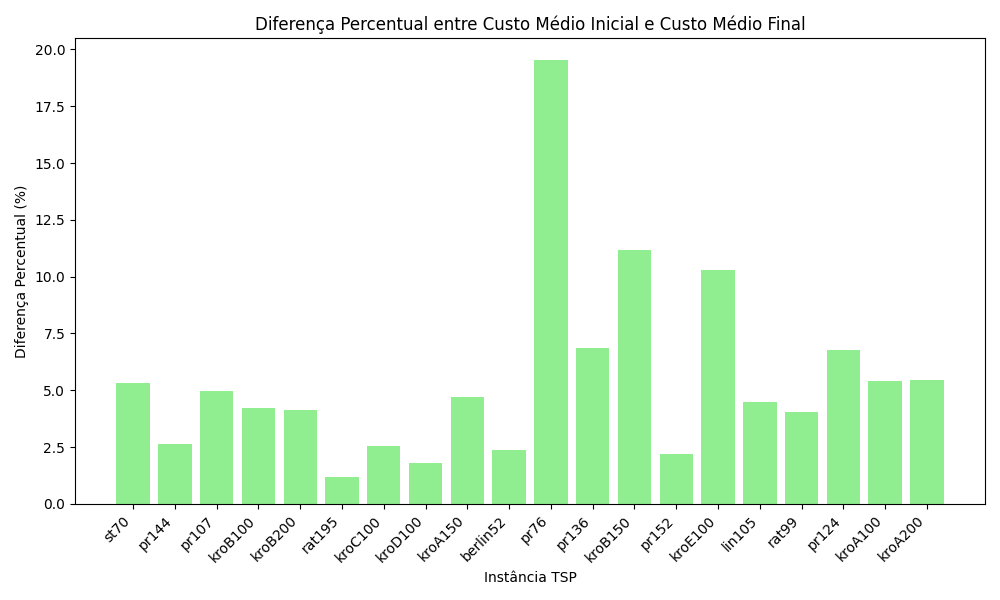
\includegraphics[width=0.5\textwidth]{./plots/path_difference_saida_00_5.log.png}
    \caption{Diferença percentual solução inicial e final alpha 0 iterações 5}
    \label{fig:Diferença percentual solução inicial e final alpha 0 iterações 5}
\end{figure}


Agora variando o parâmetro alpha, temos os resultados presentes nas imagens 4 e 5 mostrando a variação obtida com alpha = 0.2 e 5 iterações. Percebe-se a diferença no tempo de execução visto na imagem 4, obtendo um tempo maior em comparação ao alpha = 0. Isso é explicado pelo fato de existir um fator aleatório na escolha da próxima cidade, com o método gastando mais tempo até chegar um ótimo local. Além disso, a influência do fator aleatório é vista também nas imagens 5 e 6, com os resultados sendo mais distantes em relação ao ótimo, além da maior diferença entre a solução inicial e final já que a escolha aleatória pode levar a soluções piores inicialmente, com a busca local levando a mais melhorias.

\begin{figure}[H]
    \centering
        \begin{minipage}{0.5\textwidth}
        \centering
        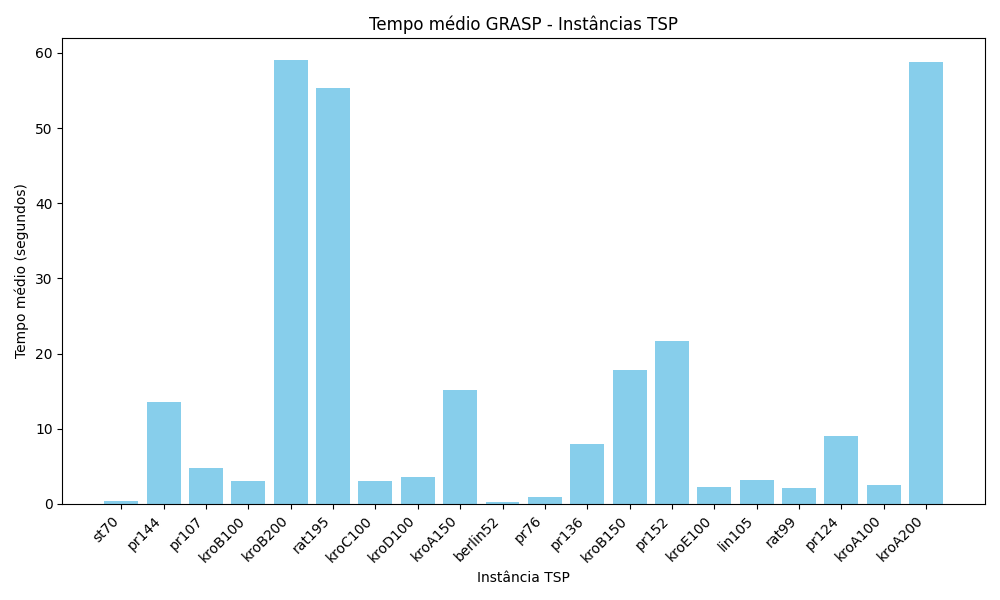
\includegraphics[width=1\textwidth]{./plots/average_times_saida_02_5.log.png}
        \caption{Tempo médio alpha 0.2 iterações 5}
        \label{fig:Tempo médio alpha 0.2 iterações 5}
    \end{minipage}\hfill
    \begin{minipage}{0.5\textwidth}
        \centering
        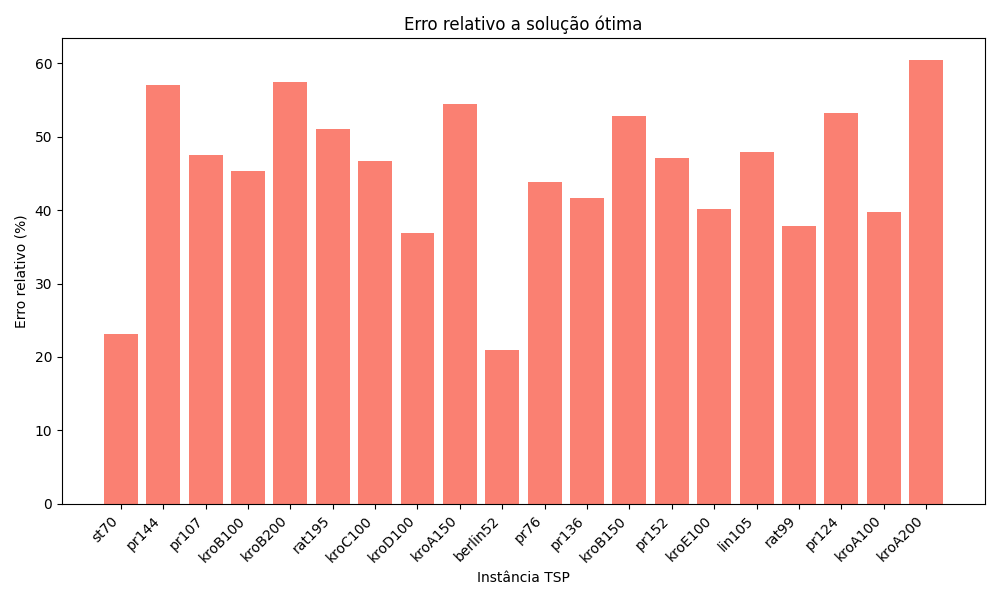
\includegraphics[width=1.0\textwidth]{./plots/solution_comparison_saida_02_5.log.png}
        \caption{Erro percentual alpha 0.2 iterações 5}
        \label{fig:Erro percentual alpha 0.2 iterações 5}
    \end{minipage}
\end{figure}

\begin{figure}[H]
    \centering
    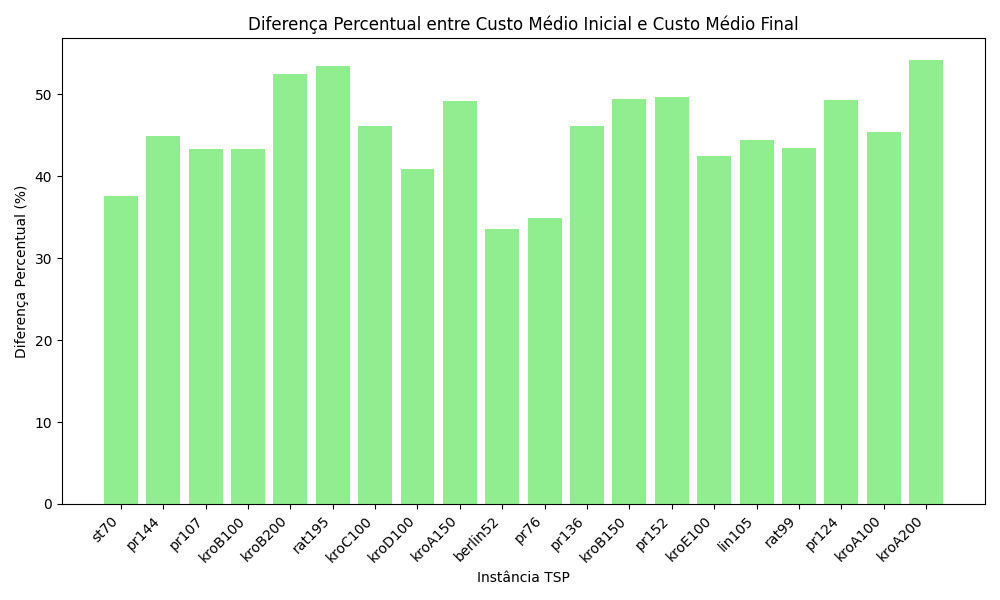
\includegraphics[width=0.5\textwidth]{./plots/path_difference_saida_02_5.log.png}
    \caption{Diferença percentual solução inicial e final alpha 0.2 iterações 5}
    \label{fig:Diferença percentual solução inicial e final alpha 0.2 iterações 5}
\end{figure}

O mesmo fato é perceptível nas imagens 7, 8 e 9 presentes abaixo, com os resultados para alpha = 0.7 e novamente com 5 iterações. Desse modo, a tendência continua, em que ao se aumentar o fator aleatório do método, piores resultados são encontrados inicialmente. Com isso, tal fato leva a maiores distâncias entre o a solução inicial e a final, além de piores resultados no erro relativo a solução ótima, visto que é mais complicado encontrar o ótimo local com a escolha aleatória das cidades.

\begin{figure}[H]
    \centering
        \begin{minipage}{0.5\textwidth}
        \centering
        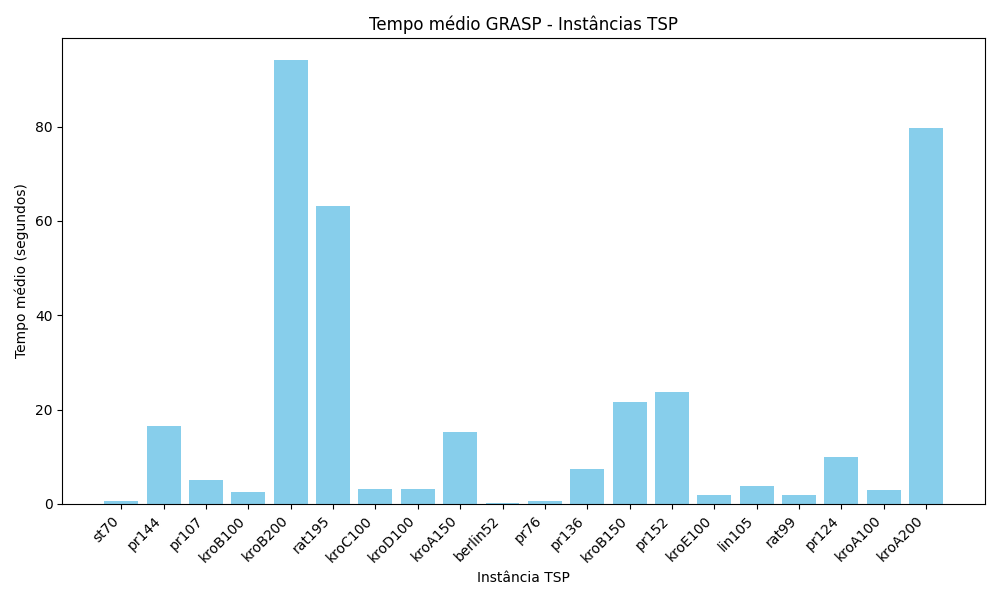
\includegraphics[width=1\textwidth]{./plots/average_times_saida_07_5.log.png}
        \caption{Tempo médio alpha 0.7 iterações 5}
        \label{fig:Tempo médio alpha 0.7 iterações 5}
    \end{minipage}\hfill
    \begin{minipage}{0.5\textwidth}
        \centering
        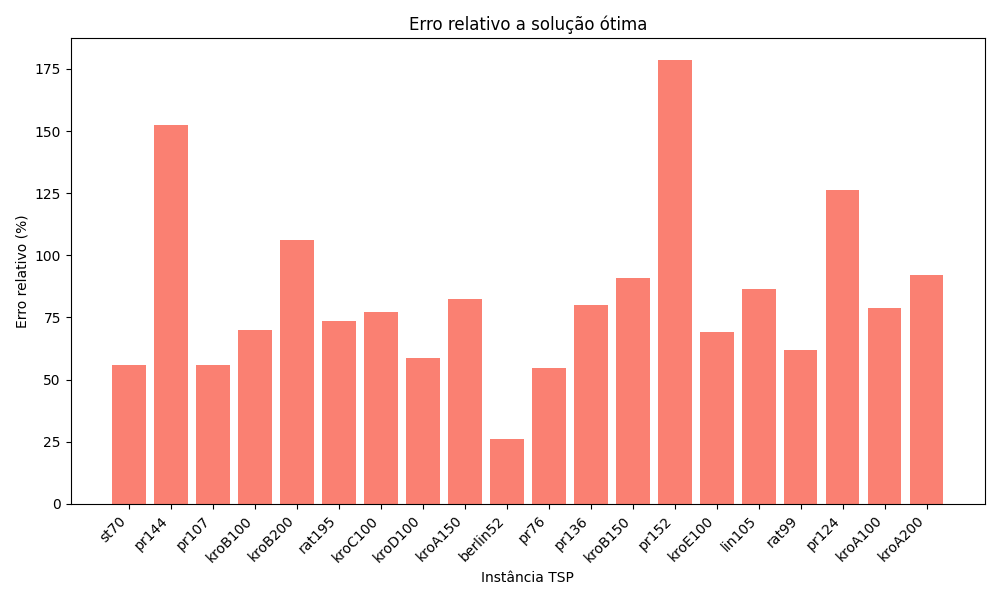
\includegraphics[width=1.0\textwidth]{./plots/solution_comparison_saida_07_5.log.png}
        \caption{Erro percentual alpha 0.7 iterações 5}
        \label{fig:Erro percentual alpha 0.7 iterações 5}
    \end{minipage}
\end{figure}

\begin{figure}[H]
    \centering
    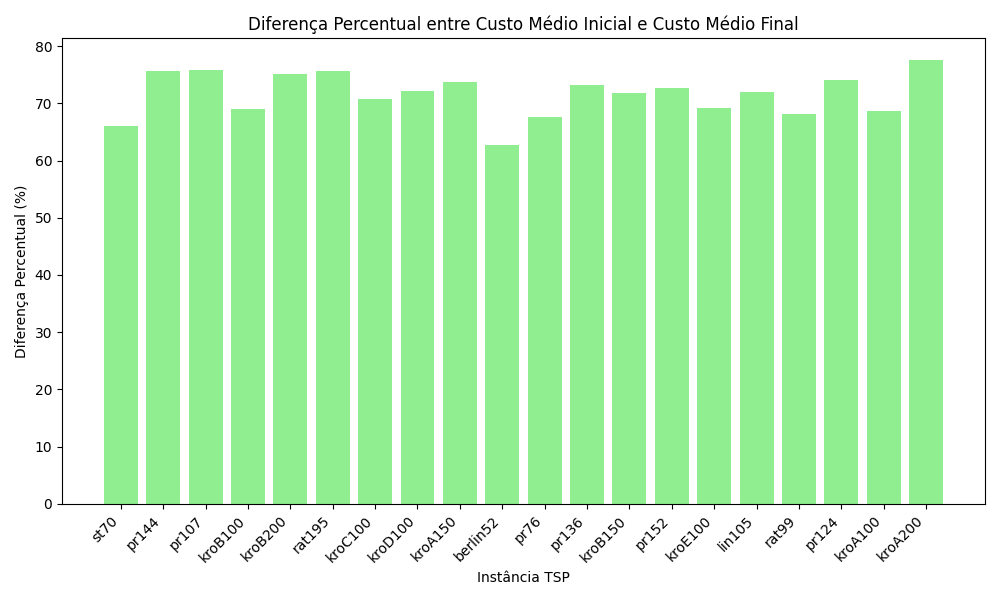
\includegraphics[width=0.5\textwidth]{./plots/path_difference_saida_07_5.log.png}
    \caption{Diferença percentual solução inicial e final alpha 0.7 iterações 5}
    \label{fig:Diferença percentual solução inicial e final alpha 0.7 iterações 5}
\end{figure}

Observando todos os resultados anteriores, a medida que mais aleatoriedade foi sendo introduzida a cada experimento, manter o número de iterações como 5 é um fator que piora os resultados para maiores valores de alpha. Desse modo, o ideal é aumentar o número de iterações do método juntamente com o aumento de alpha (isso não quer dizer que existe uma relação linear entre ambos), para assim conseguir amostrar mais soluções. Isso é válido já que, como os resultados estão mais aleatorios, a tendência é que piores soluções sejam encontradas. Assim, são necessárias mais amostras coletadas, para então boas soluções serem escolhidas ao fazer a média das execuções. Tal fato é observado nos gráficos abaixo 10, 11 e 12 em que o algoritmo foi executado com os parâmetros alpha = 0.7 e 10 iterações, em que agora os erros foram menores em relação a solução ótima já que melhores resultados foram amostrados. Já para o erro em relação aos resultados iniciais, os valores se mantêm semelhantes, visto que embora a solução final seja melhor na média, a escolha inicial também é melhor na média.

\begin{figure}[H]
    \centering
        \begin{minipage}{0.5\textwidth}
        \centering
        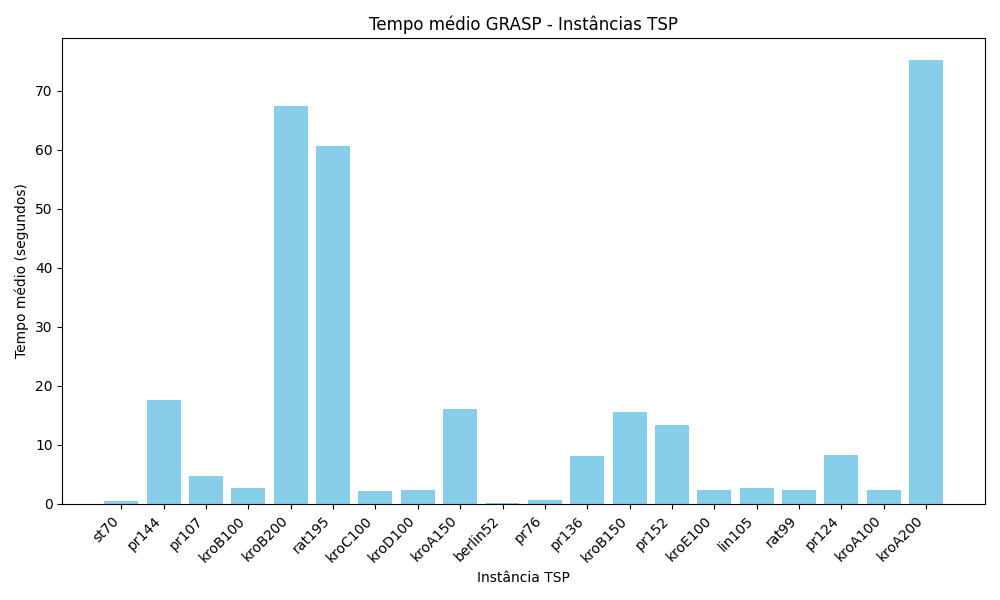
\includegraphics[width=1\textwidth]{./plots/average_times_saida_07_10.log.png}
        \caption{Tempo médio alpha 0 iterações 10}
        \label{fig:Tempo médio alpha 0 iterações 10}
    \end{minipage}\hfill
    \begin{minipage}{0.5\textwidth}
        \centering
        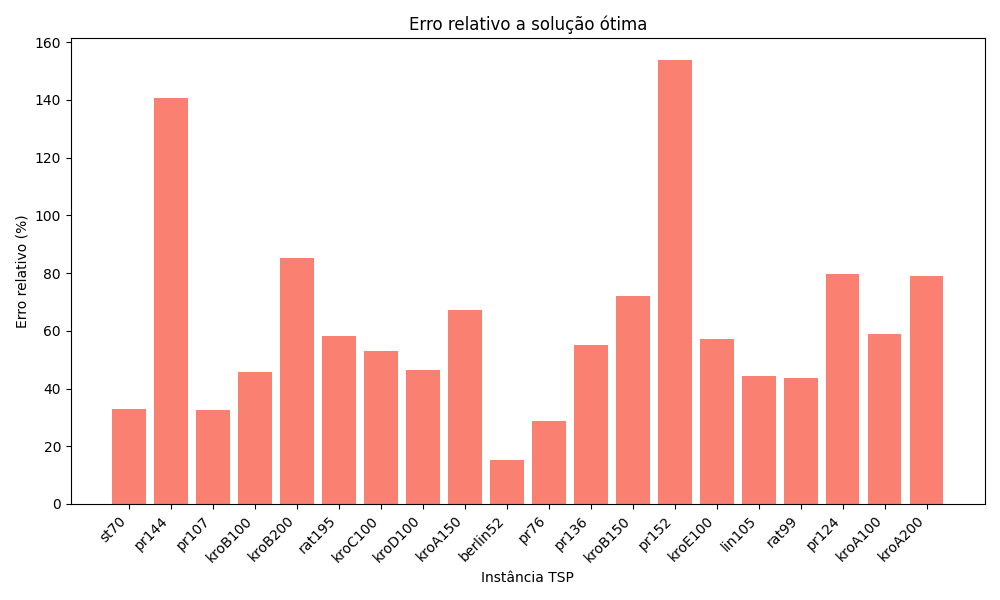
\includegraphics[width=1.0\textwidth]{./plots/solution_comparison_saida_07_10.log.png}
        \caption{Erro percentual alpha 0.7 iterações 10}
        \label{fig:Erro percentual alpha 0.7 iterações 10}
    \end{minipage}
\end{figure}

\begin{figure}[H]
    \centering
    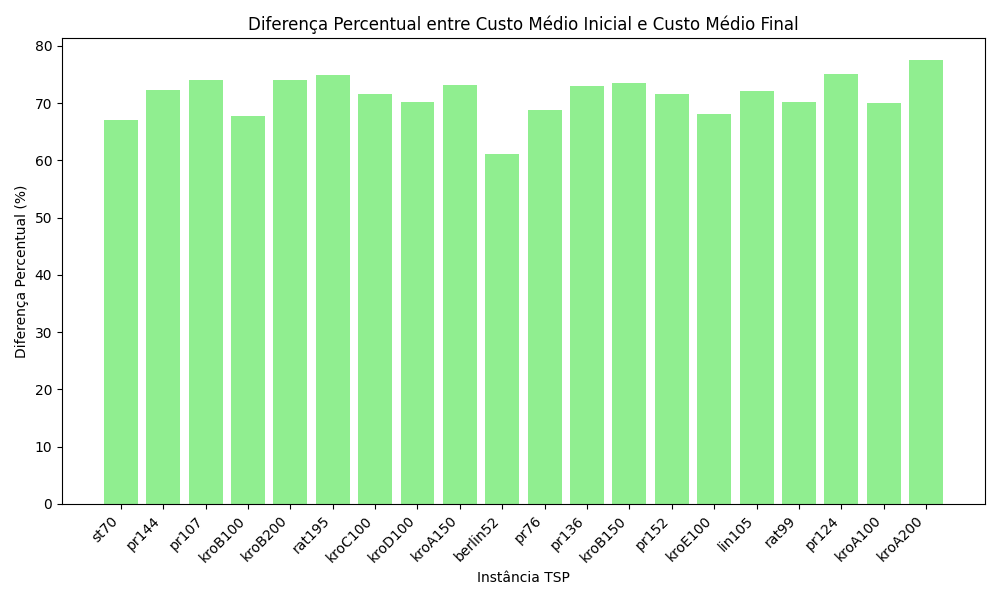
\includegraphics[width=0.5\textwidth]{./plots/path_difference_saida_07_10.log.png}
    \caption{Diferença percentual solução inicial e final alpha 0.7 iterações 10}
    \label{fig:Diferença percentual solução inicial e final alpha 0.7 iterações 10}
\end{figure}

\section{Conclusão}

Observando os resultados presentes na tabela acima, percebe-se como o método GRASP é útil e importante em problemas com um grande espaço de busca, conseguindo amostrar diferentes soluções, chegando em resultados diversos e também, dado tempo suficiente, com uma faixa aceitável de erros. Vale destacar a necessidade de aumentar o número de iterações, além de métodos de busca local mais eficientes a medida que o parâmetro alpha aumenta, visto que a escolha aleatória das cidades pode levar a soluções piores inicialmente, com a busca local sendo essencial para melhorar as soluções. Desse modo com soluções inicias piores, mais vizinhos devem ser explorados para encontrar resultados melhores, sendo mais custoso e demorado realizar tais ações a medida a busca inicial fica menos gulosa. Com isso, para futuros trabalhos tais fatores podem ser explorados para melhorar os resultados obtidos.

\section{Referências}

\noindent \href{https://www2.imm.dtu.dk/courses/02719/grasp/grasp.pdf}{GRASP – A speedy introduction}

\noindent \href{http://comopt.ifi.uni-heidelberg.de/software/TSPLIB95/}{Site com instâncias e ótimos de TSP}

\end{document}